%% ============================================================
\chapter{Methods}
\label{ch:method}
%% Target length: ~15 pages
%% Core technical contribution chapter.
This chapter describes our contributions to this thesis.
Background described the base architectures and components of MISRGRU 
and TR-MISR in
Sections~\ref{sssec:misrgru_bg} and~\ref{sssec:trmisr_bg}.

Here we describe only what is new: the modifications made when adapting model architectures to
fluorescence microscopy, an improved Transformer fusion module, a streaming variant of MISRGRU,
and a motion augmentation training strategy.




% The model is formulated as a function composition:
% \begin{equation}
%   \hat{\mathbf{Y}} = \mathcal{D}_\beta \circ \mathcal{F}_\alpha \circ \mathcal{E}_\theta(\{\mathbf{l}_1, \ldots, \mathbf{l}_N\}),
% \end{equation}
% where $\mathcal{E}_\theta$, $\mathcal{F}_\alpha$, and $\mathcal{D}_\beta$ are the encoder, fusion, and decoder modules with trainable parameters $\theta$, $\alpha$, and $\beta$ respectively. Each module serves a distinct role:

% \begin{enumerate}
%   \item \textbf{Encoder} $\mathcal{E}_\theta$: extracts spatial features and structural information from each of the $N$ input frames independently, producing encoded representations $\{\mathbf{r}_1, \ldots, \mathbf{r}_N\}$.
  
%   \item \textbf{Fusion} $\mathcal{F}_\alpha$: aggregates cross-frame information by identifying correlations in the blinking statistics across all $N$ frames, producing a single latent vector $\mathbf{z}$ that summarises the multi-frame context.
  
%   \item \textbf{Decoder} $\mathcal{D}_\beta$: upsamples the fused representation to the target resolution $(2H - 7) \times (2W - 7)$ and produces the final SR image $\hat{\mathbf{Y}}$.
% \end{enumerate}

% The following sections detail each module and the key design choices that differentiate this work from prior approaches.


\section{Modifications to TRMISR}
\label{sec:adaptation}

\paragraph{Encoder.}
Our modified TRMISR shares the same encoder design as RESURF~\cite{resurf2024}. 
The original TR-MISR encoder takes a two-channel input formed by concatenating
  each
  grayscale low-resolution frame with a median reference
  image. In TR-MISR the median reference serves as an
  implicit co-registration anchor and a shared representation for separating redundant
  content from
  frame-unique detail~\cite{TR-MISR-original}.

We drop the median reference and use a single-channel input.
  Removing the median does not discard the information that drives
  super-resolution. The
  resolution gain in SOFI comes from the blinking-induced intensity
fluctuations across the frame ensemble. 

This is tested out empirically: an ablation that concatenates an averaged
  reference image as a second encoder channel is significantly worse than the
  single-channel model across every imaging condition and on every paired test
  sample ($\overline{d} = +0.027$ RSP pooled in favour of the single channel,
  $p \approx 2.3\times10^{-80}$, rank-biserial $=-1.00$), with the gap widening
  as the blinking slows and the photon count drops
  (Appendix~\ref{app:encoder_ablation}).

We reduce the encoder width from 64 to 24 channels.
Reducing the encoder width from 64 to 24 channels roughly halves inference latency at every
frame count (e.g.\ 226\,ms vs.\ 436\,ms at 20 frames for 512x512 input images), 
while costing only a small drop in reconstruction quality (aggregate RSP
$0.8925$ vs.\ $0.8955$, a statistically significant but minor $0.003$ decrease that widens to
$0.006$ in the hardest slow-blinking, low-SNR condition).
We therefore use the 24-channel encoder for all fusion-mechanism comparisons, both to match
the RESURF configuration~\cite{resurf2024} and because the latency saving outweighs the
marginal quality loss; the wider 64-channel encoder is preferable when quality is prioritised.

\paragraph{Decoder.}
The original TR-MISR decoder uses a $3\times$ PixelShuffle~\cite{shi2016pixelshuffle,zhuocen2023espcn} for the
$3\times$ upscaling.
PixelShuffle (sub-pixel convolution) rearranges the channels of a low-resolution feature map
of shape $(C\cdot r^2, H, W)$ into a high-resolution map of shape $(C, rH, rW)$, performing the
upscaling by an integer factor $r$ without learnable upsampling parameters (Figure~\ref{fig:pixelshuffle}).
For the $(2H-7)\times(2W-7)$ SOFI upscale, we compare two decoder designs:
a $2\times$ PixelShuffle followed by a centre-crop to match the target resolution,
 and a learned transposed convolution that achieves the exact
 $(2H-7)\times(2W-7)$ output size directly.
These are described in detail in Section~\ref{sec:decoder}.

\begin{figure}[htbp]
  \centering
  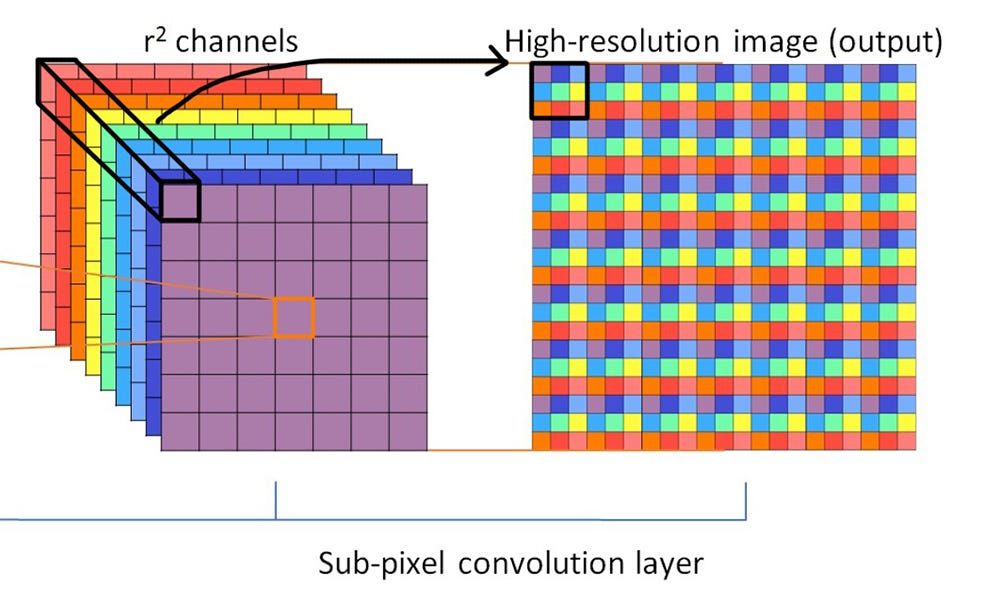
\includegraphics[width=\linewidth]{figures/pixelshuffle.jpg}
  \caption{PixelShuffle (sub-pixel convolution) upscaling by a factor $r$: the
  $(C\cdot r^2, H, W)$ feature map is rearranged into a $(C, rH, rW)$ high-resolution
  output~\cite{shi2016pixelshuffle,zhuocen2023espcn}.}
  \label{fig:pixelshuffle}
\end{figure}

% \paragraph{Positional encoding.}
% The original TR-MISR fusion is has no positional encoding on the frame
% tokens (Section~\ref{sssec:trmisr_bg}). This works well in satelite domain because the input
% images are not in sequence and the order does not matter.

% In fluorescent microscopy domain and SOFI specifically exploits temporal fluctuations in pixels.
% For this reason we add a learnable frame-index positional embedding to the token sequence before the
% first Transformer layer, so the model can exploit the temporal order of blinking events.

\section{Improved Fusion}
\label{sec:fusion}

The base TR-MISR fusion module is described in Section~\ref{sssec:trmisr_bg}, but in short
it pays attention to encoded input frames by fusing the information into an additional learnable embedding
vector.
For every pixel $(h,w)$, in the sequence of $N$ frames:
the embedding token $x^0$ is prepended (Eq.~\eqref{eq:trmisr_z0}), and after $M$
Transformer layers the token at index~0 is extracted as the fused feature (Eq.~\eqref{eq:trmisr_msa}--\eqref{eq:trmisr_ffn}).
We identified two problems with this design and propose fixes for both.

\subsection{Problem 1: Attention Scaling Bug}

The original TR-MISR code scales attention scores by $1/\sqrt{d_\mathrm{model}}$, where
$d_\mathrm{model}$ is the full embedding dimension.
The standard~\cite{vaswani2017attention} is to scale by $1/\sqrt{d_k}$, where
$d_k = d_\mathrm{model}/q$ is the per-head dimension.
The two differ by a factor of $\sqrt{q}$, meaning attention logits are under-scaled,
which pushes the softmax towards a uniform distribution, every frame receives roughly
equal weight regardless of its signal quality.

We replace the manual attention implementation with \texttt{nn.MultiheadAttention}%
\footnote{\url{https://docs.pytorch.org/docs/stable/generated/torch.nn.MultiheadAttention.html}},
which applies the correct $1/\sqrt{d_k}$ scaling internally.
However, this bug only affects multi-headed attention. In the final TRMISR design 
we use single head, and single depth attention fusion mechanism, since our ablation study shows
that increasing 
the number of heads and attention depth increases latency without significantly improving accuracy.

\subsection{Problem 2: Class Token replaced with CrossAttentionAggregator}

In the original TR-MISR, a single learnable class token is added into the self-attention sequence
together with the $N$ frame tokens.
This token is expected to do two things at once: help the frame tokens exchange information with
each other, and collect the final fused representation.

\textbf{CrossAttentionAggregator.}
We separate the two roles.
First, the $N$ frame tokens attend to each other through self-attention layers without the class
token, thus all information is used for frame-to-frame communication.
Then a single learned query vector $\mathbf{Q}$ cross-attends to the updated frame tokens to
produce the fused feature:
\begin{equation}
  \mathbf{z}^u = \mathrm{CrossAttn}\!\left(\mathbf{Q},\; \{x^1,\ldots,x^k\}\right).
  \label{eq:crossattn}
\end{equation}
The full forward pass is therefore: (1) add positional embeddings to the frame tokens;
(2) run $M$ self-attention layers on the frame tokens only;
(3) aggregate with the cross-attention query to obtain $\mathbf{z}^u$;
(4) decode $\mathbf{z}^u$ to the SR output.
The CrossAttentionAggregator is similar to attention-based 
pooling (PMA) in Set Transformer\cite{lee2019set_transformer}, 
which has been shown to outperform fixed pooling strategies for set 
representation learning tasks.

\section{PixelShuffle vs Convolutional decoder}
\label{sec:decoder}

The decoder receives a fused spatial feature map $\mathbf{z} \in \mathbb{R}^{C \times H \times W}$
and must produce the target SOFI image $\hat{\mathbf{Y}} \in \mathbb{R}^{1 \times (2H-7) \times (2W-7)}$.
Two decoder designs were compared to handle this non-integer upscaling.

\paragraph{PixelShuffle decoder (TR-MISR baseline).}
PixelShuffle~\cite{shi2016pixelshuffle}, is an efficient and parameter-free
spatial upsampler \cite{TR-MISR-original}. It rearranges feature channels from a low-resolution feature map 
into higher-resolution output. Moreover, this approach avoids the checkerboard artefacts that 
transposed convolutions can introduce when their stride does not divide evenly into the kernel size 
\cite{odena2016deconvolution}.
More specifically, let the input feature map have dimensions $H \times W \times C_{\text{in}} r^2$, 
where $r$ is the upscaling factor. The pixel shuffle operation transforms this tensor into an output 
of size $rH \times rW \times C_{\text{in}}$ by redistributing the $r^2$ channels associated 
to each spatial location into an $r \times r$ spatial neighborhood in the high-resolution image.

For the PROBA-V satellite benchmark, the target resolution was an exact $3\times$ upscale of the input. 
We modified the original network for our use case, so a $2\times$ PixelShuffle is applied.
Our decoder consists of the following steps:
\begin{enumerate}
  \item A $3 \times 3$ convolutional layer with PReLU activation decreases the number of channels from $24$ to $4C$.
  \item PixelShuffle rearranges the 
  $4 \times H \times W$ tensor into $1 \times 2H \times 2W$.
  \item A centre-crop operation removes 3 pixels from the top/left and 4 pixels from the bottom/right, which results in the desired output size.
\end{enumerate}
The crop introduces a asymmetric offset in the predicted image and 
does not back-propagate any learnable upsampling signal through the cropped region. 
This is a known limitation of PixelShuffle when the target size is not an exact power-of-two multiple of the input.

\paragraph{ConvTranspose2d decoder (TRNet\_deconv and MISRGRU).}
The original MISRGRU~\cite{MISRGRU-original} and RESURF~\cite{resurf2024} models use a
transposed convolutional layer to upsample the fused features. The key advantage over PixelShuffle is that the
upsampling kernel is fully learned and the $2H - 7$ target size is achieved without any explicit crop,
so the decoder's receptive field covers all output pixels:
\begin{equation}
  \hat{\mathbf{Y}} = \mathcal{D}_\beta(\mathbf{z}) \in \mathbb{R}^{1 \times (2H-7) \times (2W-7)}.
  \label{eq:decoder}
\end{equation}

The decoder consists of the following layers:
\begin{enumerate}
  \item \texttt{ConvTranspose2d}($C \to C$, kernel $3\times3$, stride 2, padding 4, output\_padding 0)
  \item Two $3 \times 3$ convolutional layers with PReLU refine the upsampled features.
  \item A $1 \times 1$ convolutional projection reduces from $C$ channels to a single output channel.
\end{enumerate}
All three layers maintain $C = 24$ channels until the final projection.

The output spatial dimension of a transposed convolution with kernel size $k$, stride $s$, padding $p$, and output padding $p_\text{out}$ is:
\begin{equation}
  H_\text{out} = (H_\text{in} - 1) \cdot s - 2p + k + p_\text{out}.
  \label{eq:convtranspose_size}
\end{equation}
Substituting the decoder parameters ($s{=}2,\ p{=}4,\ k{=}3,\ p_\text{out}{=}0$) gives:
\begin{equation}
  H_\text{out} = (H - 1)\cdot 2 - 2\cdot 4 + 3 = 2H - 7,
  \label{eq:decoder_size}
\end{equation}
which matches the 2nd-order SOFI target exactly.


\section{Optimizing MISRGRU}
\label{sec:optimizing_misrgru}

The original MISRGRU model (Section~\ref{sssec:misrgru_bg}) takes a fixed set of $N$ input frames and outputs
a single SR image.
This has two limitations for real-time live-cell imaging.
First, for every new incoming frame the entire $N$-frame sequence must be re-encoded and re-processed
from scratch, which is redundant since the ConvGRU hidden state $\mathbf{h}_N$ already encodes a
summary of all previous frames.
Second, the batch model is many-to-one: it produces one output per $N$ input frames.
To super-resolve a full movie, the entire sequence would need to be processed in rolling windows which
again introduces the computational redundancy.

This section develops a family of MISRGRU variants that progressively address these
limitations. Table~\ref{tab:misrgru_variants} previews all six models, their architectural
modifications, and how they are trained; each is described in detail in the subsections that
follow and evaluated in Chapter~\ref{ch:results}.

\begin{table}[htbp]
  \centering
  \caption{Overview of the MISRGRU model variants studied in this thesis. The output mode
  $N{\to}1$ denotes one SR image per $N$ input frames (batch); $N{\to}N$ denotes one SR
  output per incoming frame (streaming). All streaming variants reuse the encoder and decoder
  of the batch model and differ only in hidden-state handling, added modules, and training.}
  \label{tab:misrgru_variants}
  \small
  \begin{tabularx}{\linewidth}{@{}l c X X@{}}
    \toprule
    \textbf{Model} & \textbf{Output} & \textbf{Modification} & \textbf{Training strategy} \\
    \midrule
    Batch MISRGRU (foundational) & $N{\to}1$  &
    RESURF\cite{resurf2024} ConvGRU baseline; GAP aggregates all hidden states $h_1\dots h_N$;
    state reset per sample. &
    Fourier loss on model output and SOFI target.\\
    \addlinespace
    Sliding-window MISRGRU & $N{\to}N$ &
    Circular buffer of the last $n$ hidden states; hidden states are cached only $n$-th is computed. 
    GAP aggregates only the windowed states before decoding. &
    No training needed, reuses weights from the Batch MISRGRU. \\
    \addlinespace
    Streaming MISRGRU & $N{\to}N$ &
    GAP module removed; decoder reconstructs from the last hidden state $h_k$ alone; state
    never reset. Ability to aggregate more information over time. &
    Truncated BPTT (TBPTT) with chunking and \texttt{loss\_last\_n} supervision; Fourier loss. \\
    \addlinespace
    Larger GRU & $N{\to}N$ &
    Streaming MISRGRU with increased ConvGRU hidden-state capacity (95k\,$\to$\,131k params). &
    Trained from scratch with TBPTT ($\approx$190 epochs, DelftBlue); gives best static accuracy. \\
    \addlinespace
    Fine-tuned MISRGRU & $N{\to}N$ &
    Streaming MISRGRU architecture, no new modules. &
    Initialised from baseline Fourier weights and fine-tuned for 100 epochs on
    motion-augmented data. \\
    \addlinespace
    MISRGRU with DPA & $N{\to}N$ &
    Adds a Deformable Phase-space Alignment module (RFFT phase correction + deformable
    convolution) that aligns $h_{t-1}$ to $f_t$ before the recurrent update. &
    Zero-initialised module fine-tuned from baseline Fourier weights for 300 epochs on
    motion-augmented data. \\
    \bottomrule
  \end{tabularx}
\end{table}

\subsection{Converting MISRGRU to many-to-many}
\label{sec:streaming_arch}
An architecture where many inputs produce many outputs would address both
problems: one SR image is produced per incoming frame, 
and the GRU hidden state is carried across frames rather than reset between batches. 
This way the model could accumulate more information from input frames,
which can help to better reconstruct, while keeping the latency low per
reconstructed image.


\subsubsection{Sliding-window MISRGRU}
A circular buffer of the last $n$ hidden states is maintained across time steps. 
At each step $k$, the encoder processes the incoming frame 
$\mathbf{I}_t$, the ConvGRU updates its state, and the GAP module 
aggregates features from the last $n$ hidden states before decoding to produce 
$\hat{\mathbf{Y}}_t$. 
This design retains the multi-frame fusion capability of batch MISRGRU while 
enabling streaming inference without resetting the hidden state every K frames, while
also saving compute by remembering $h_{k-n} \dots h_{k-1}$.

We designed experiments in section~\ref{ssec:kbuf_misrgru} to see how this architecture without 
reinitializing the hidden state performs when run longer than 20 frames. 
The results from the experiments prompted us to remove the GAP layer and force the 
Decoder to reconstruct the SR output only from last hidden state $h_k$.

\begin{figure}[htbp]
  \centering
  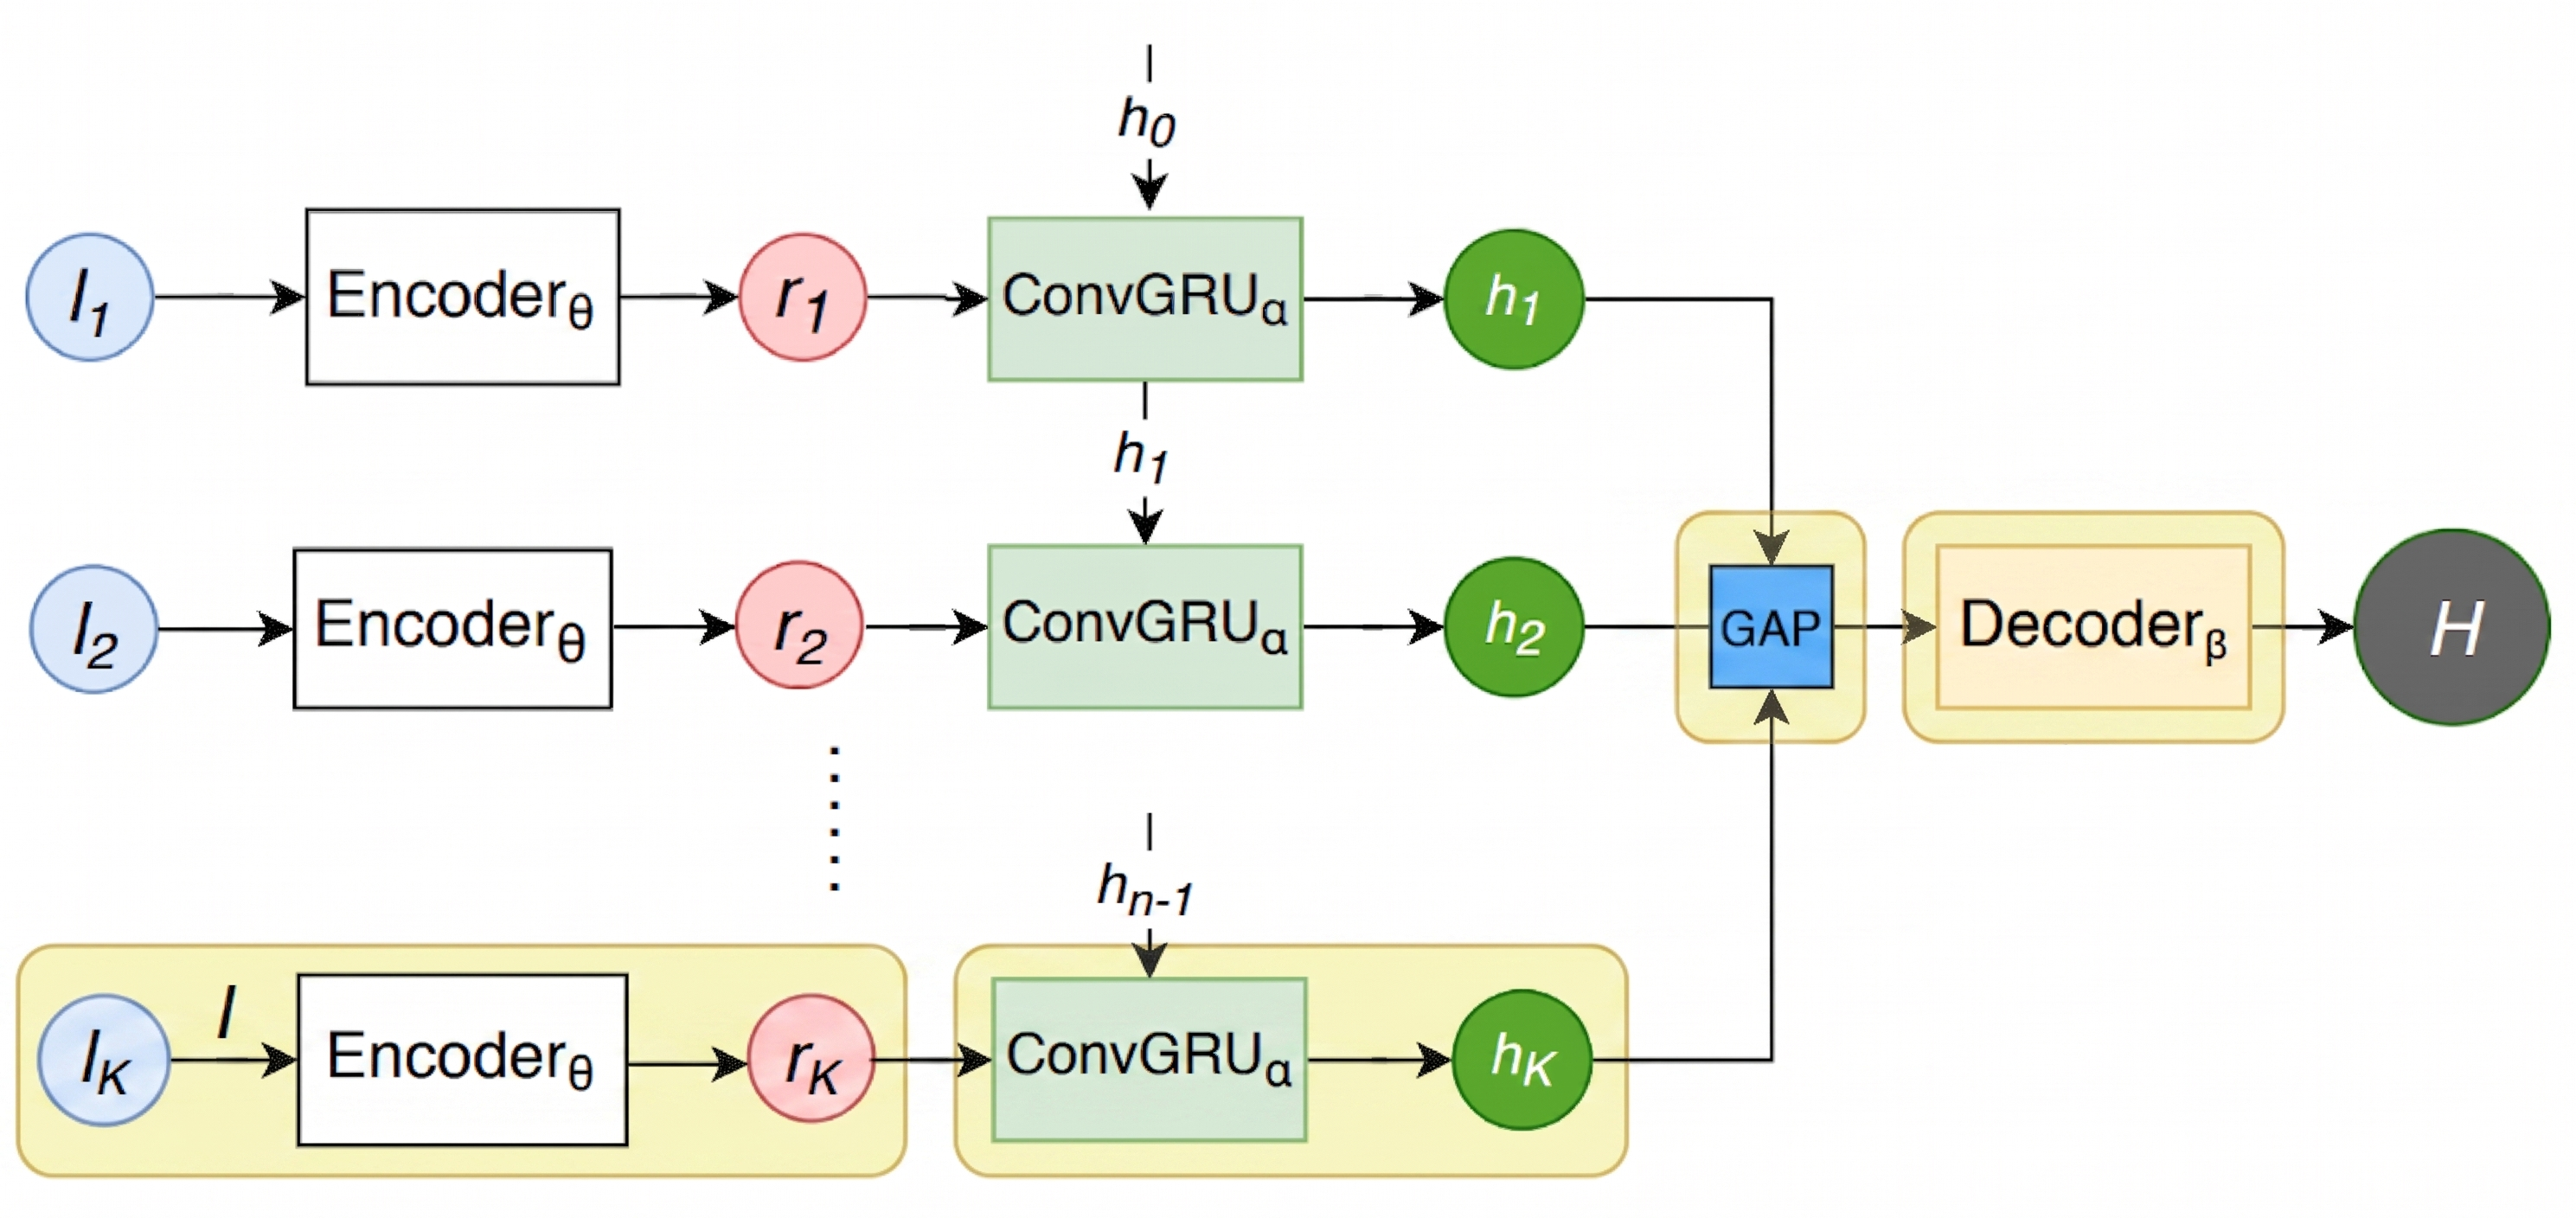
\includegraphics[width=\linewidth]{figures/sliding_window_misrgru.png}
  \caption{Sliding-window MISRGRU architecture. Only highlighted parts are being 
  computed at arrival of new input frame. ConvGRU outputs $h_{k-n} \dots h_{k-1}$ are
  being stored in circular buffer for faster inference}
  \label{fig:sliding_window_arch}
\end{figure}

\subsubsection{Removing the GAP module}
The Streaming MISRGRU (Figure~\ref{fig:streaming_arch}) reuses the encoder and decoder from the
batch MISRGRU without modification.
The only architectural change is in how the ConvGRU hidden state is managed.
In the batch model, the hidden state is zeroed at the start of each new sample.
In the streaming model, $\mathbf{h}_t$ is carried across successive frames and never reset
between time steps, so the GRU accumulates context from the entire history of frames seen so far.
The GAP in RESURF\cite{resurf2024} is computed as sum of all $h_{1} \dots h_{k}$.
Removing it forces both ConvGRU and Decoder to reconstruct the SR output from last hidden 
state $h_k$ at every new frame.


\begin{figure}[htbp]
  \centering
  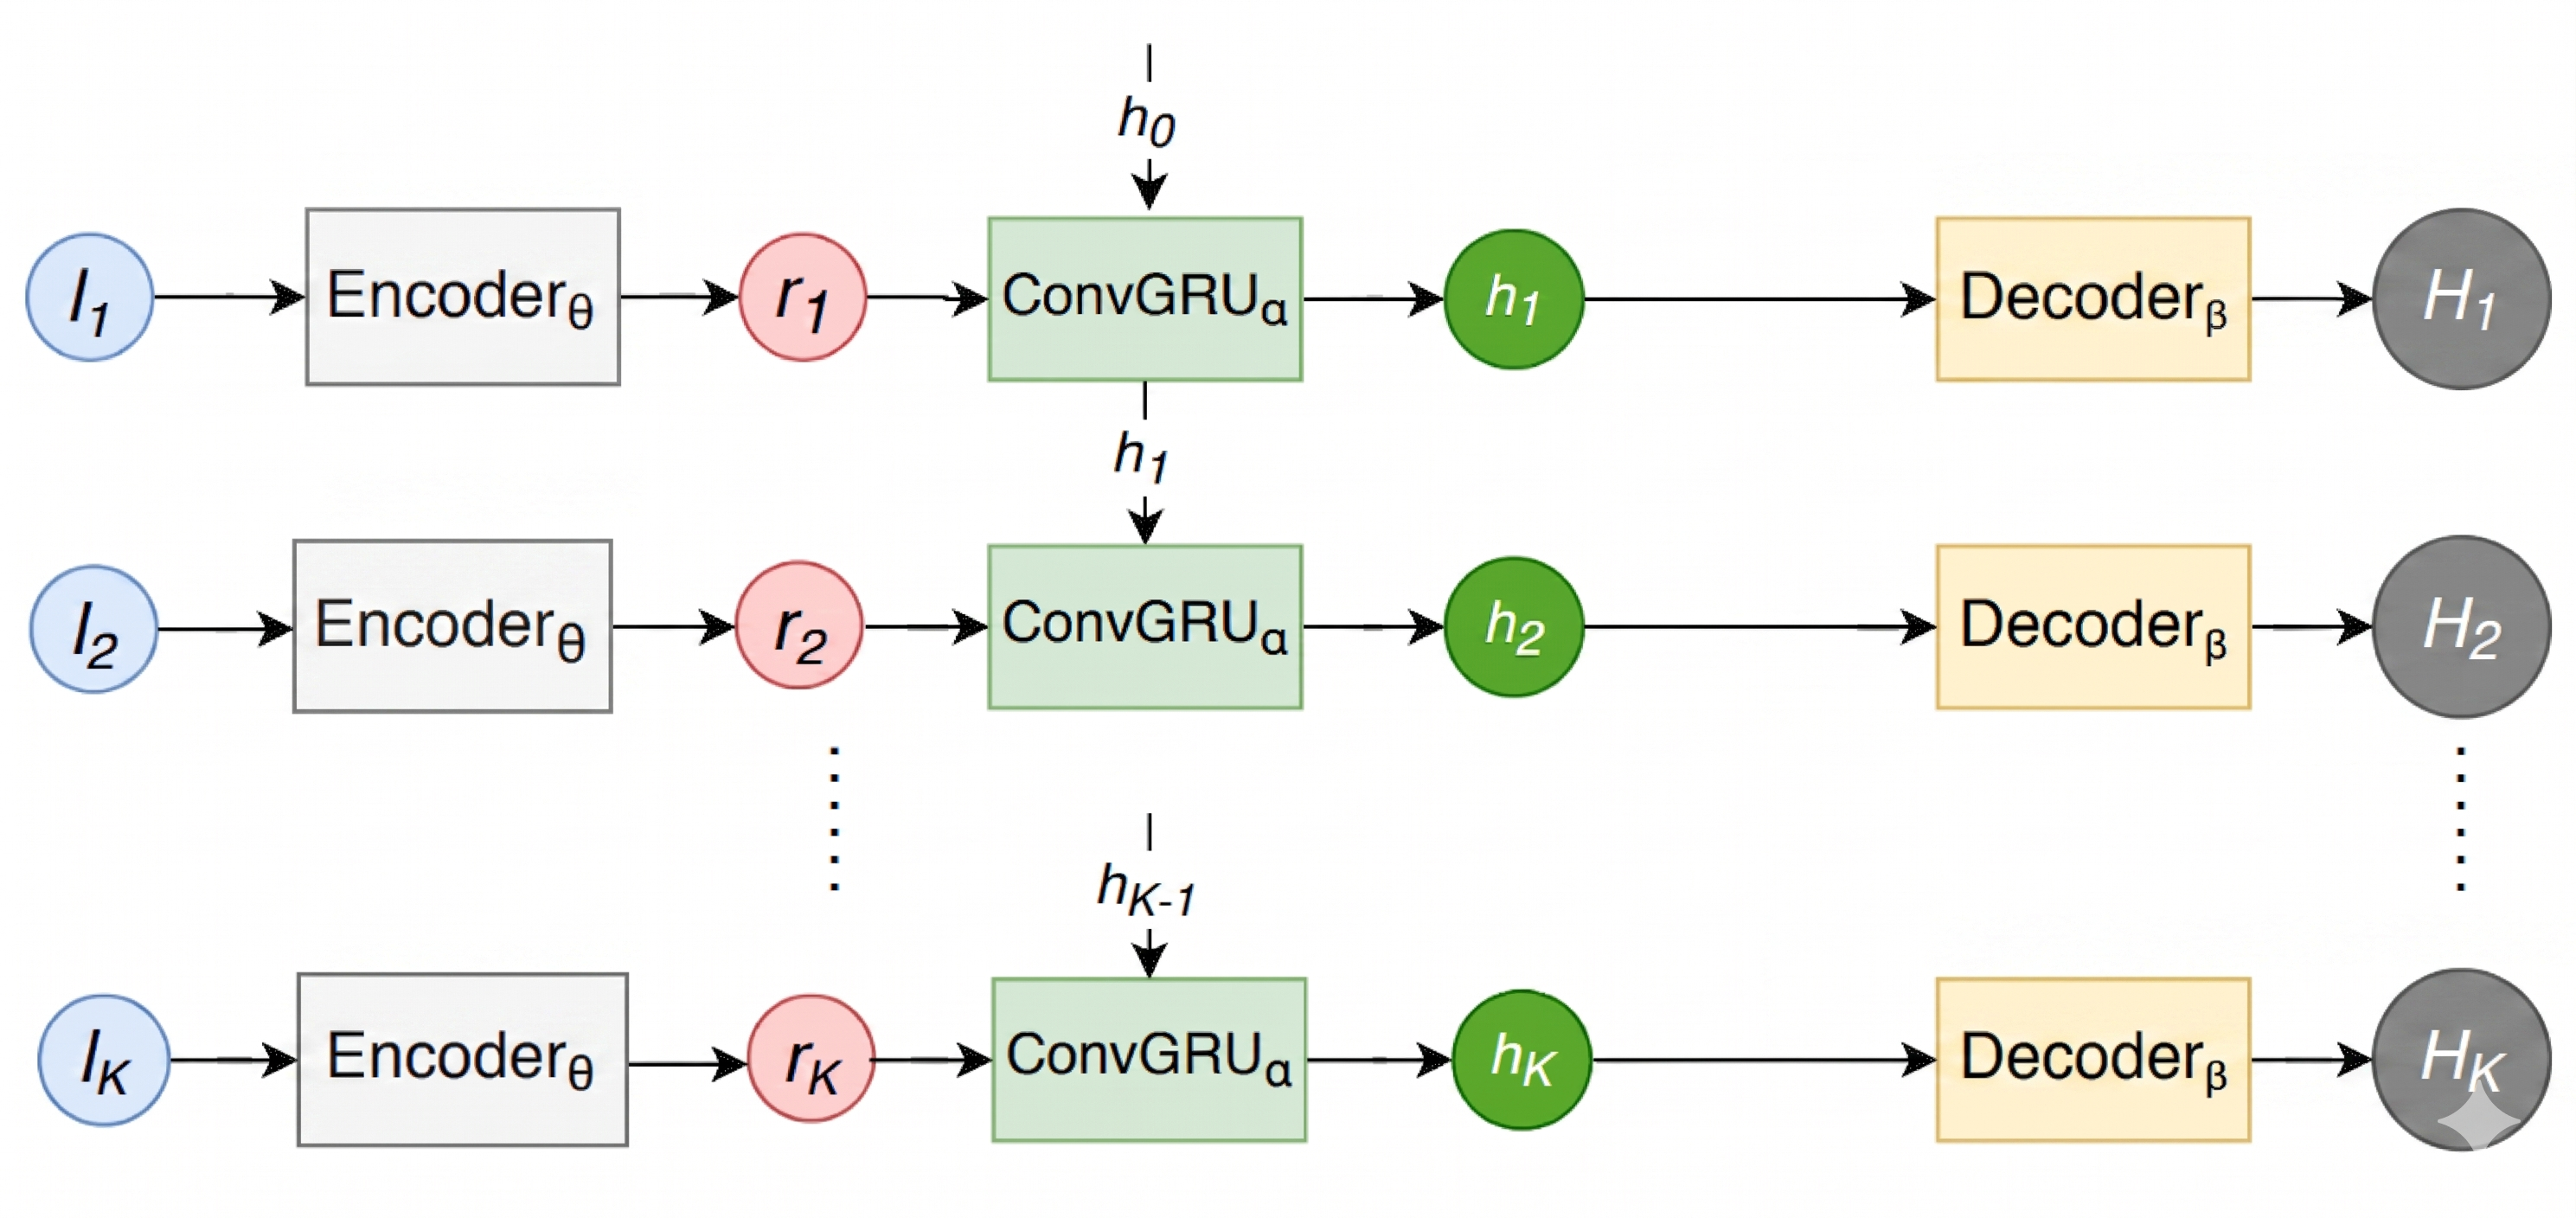
\includegraphics[width=\linewidth]{figures/streaming_misrgru_architecture.png}
  \caption{Streaming (many-to-many) MISRGRU architecture. 
  Each input frame $\mathbf{l}_t$ is encoded by the shared encoder, 
  fused by the ConvGRU with the previous hidden state 
  $\mathbf{h}_{k-1}$, and decoded to produce the SR output $\hat{\mathbf{Y}}_t$ at every time step.}
  \label{fig:streaming_arch}
\end{figure}

% \begin{equation}
%   \mathbf{h}_t = \text{ConvGRU}(\text{Encoder}(\mathbf{l}_t),\ \mathbf{h}_{t-1}),
%   \qquad
%   \hat{\mathbf{Y}}_t = \text{Decoder}(\mathbf{h}_t).
%   \label{eq:streaming}
% \end{equation}

\subsubsection{Training with Truncated Backpropagation through Time}

Training on sequences of length 50 frames with standard backpropagation through time 
(BPTT) is memory intense: the activation graph grows linearly with sequence length. 
To solve this we \emph{truncated BPTT} (TBPTT). The sequence is split into chunks of 
length \texttt{chunk\_size}, and the hidden state is detached from the computational graph at each 
chunk boundary. Only gradients within a chunk are backpropagated. 
Moreover this helps the model to stabilize, train faster for more epochs and trains model to learn from 
warm state when hidden state is detached, which resembles a real-world scenario during long inferences.

A second key hyperparameter is \texttt{loss\_last\_n}: supervision is applied only on the 
\emph{last} $n$ frames of each chunk, allowing the GRU to accumulate meaningful context for 
several steps before being penalised. Supervising every frame from the first step (as in the 
\texttt{loss\_all\_frames} variant) causes the model to optimise for single-frame output 
quality, which prevents the GRU from learning to defer quality improvements to later frames.


\subsubsection{Deformable Phase-space Alignment modification(DPA)}
\label{sssec:dpa}
% \todo{add figure explaining DPA}

In live-cell imaging, the imaged structure can drift between frames, meaning
$\mathbf{h}_{t-1}$ may encode a field of view that has shifted relative to the
current encoder features $\mathbf{f}_t$.
Passing a misaligned hidden state directly into the ConvGRU introduces ghosting
artefacts and degrades reconstruction quality.
To address this, we add a two-stage \emph{Deformable Phase-space Alignment} (DPA)
module that maps $\mathbf{h}_{t-1}$ into the coordinate system of $\mathbf{f}_t$
before the recurrent update, following the DPA-TISR\cite{qiao2025dpatisr} alignment order.

\paragraph{Stage 1: Frequency-domain phase correction (\texttt{RFFTAlignment}).}
Global sub-pixel drift looks as a phase shift in the 2D frequency domain.
Both $\mathbf{h}_{t-1}$ and $\mathbf{f}_t$ are transformed with the real-valued FFT,
and a small CNN predicts a per-channel phase correction from their concatenated phase
spectra.
This delta is added to the phase of $\mathbf{h}_{t-1}$ while its amplitude is kept
unchanged, after which the corrected hidden state $\mathbf{h}_\phi$ is recovered via
the inverse FFT.

\paragraph{Stage 2: Deformable convolution for local correction (\texttt{DeformableConvAlignment}).}
Residual non-rigid deformations are handled by a deformable convolution stage.
A second CNN predicts per-pixel sampling offsets and from the
concatenated pair $[\mathbf{h}_\phi,\, \mathbf{f}_t]$.
The offsets warp the sampling grid of a $3{\times}3$ convolution applied to
$\mathbf{h}_\phi$, while the masks gate each sample point, allowing the network to
suppress unreliable aligned regions.
The resulting $\mathbf{h}_\text{aligned}$ is passed to the ConvGRU together with the
$\mathbf{f}_t$, so the SR output remains anchored to the current
frame rather than a stabilised reference.

\paragraph{Zero-initialisation and first-frame behaviour.}
The output layers of both alignment CNNs and the offset/mask head are zero-initialised,
and the deformable convolution weight is identity-initialised (centre tap set to one).
This ensures the model starts as a standard streaming GRU with no alignment applied and
learns the correction transforms progressively during training.
On the first frame, when no $\mathbf{h}_{t-1}$ is available, the DPA stage is skipped
entirely and the GRU is initialised from a zero hidden state. This way we can reuse  
trained weights and only finetune the model. Section~\ref{sec:alignment_ablation} evaluates
the reconstruction accuracy of DPA MISRGRU.

\subsection{Motion Augmentation Training}
\label{sec:motion_training}


A model trained only on static data, where every frame shows the same field of view, has no
incentive to track the current position of the sample.
In live-cell imaging, organelles can move at
0.5--5\,\textmu m/s~\cite{tang2013fast} depending on a structure. This corresponds to 
$\approx$0.05--0.5 pixels per frame, our pixel size (100\,nm) and acquisition rate of 100\,fps.

To train the streaming model to be robust to motion, we introduce \emph{motion augmentation} during
training.
For each training sequence, with probability $p = 0.7$ a sinusoidal drift trajectory is
sampled independently for each spatial axis.
Sinusoids produce smooth, bounded motion with no directional bias, and their frequency
and amplitude are sampled to keep the instantaneous speed in the range 0.2--1.5
pixels/frame.
This range intentionally exceeds the biological estimate above, providing robustness to
faster stage drift and to higher-fps acquisition settings where the same physical speed
maps to more pixels per frame.

Augmentation is applied on-the-fly: at each training step, the $256{\times}256$ source
LR frame is shifted by the trajectory displacement using bilinear interpolation, and a
fixed $180{\times}180$ center crop is extracted equivalent to sliding a crop window
across the source.
The static HR ground truth is shifted by the same displacement scaled by the upsampling
and center-cropped to the matching HR size, producing a
per-frame HR target that matches the shifted field of view.
The remaining 30\% of training sequences use the unshifted static patches, which
prevents the model from degrading on non-moving data.

\begin{figure}[htbp]
  \centering
  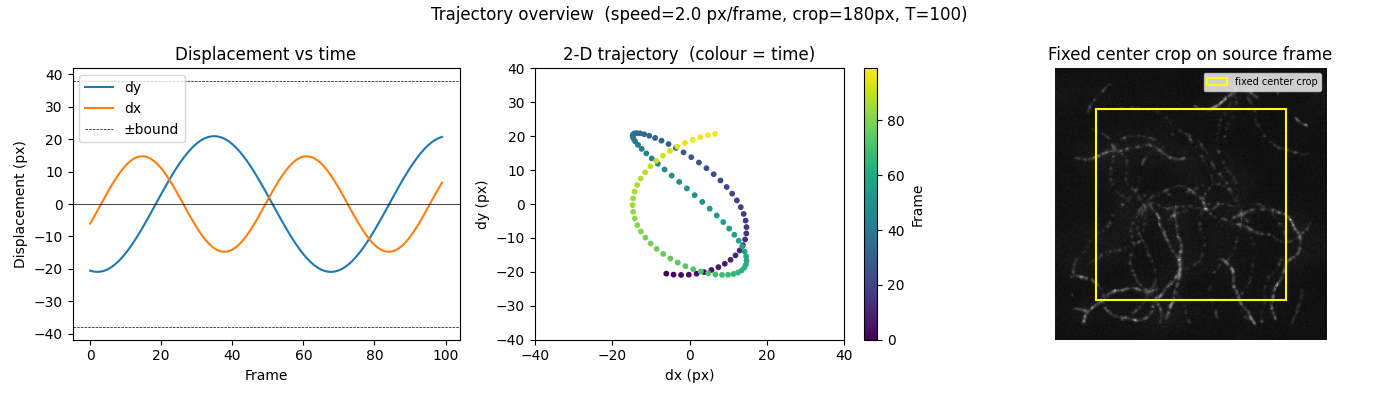
\includegraphics[width=\linewidth]{figures/motion_augmentation.png}
  \caption{Motion augmentation. A sinusoidal drift trajectory is sampled per axis and
  used to shift the $256{\times}256$ source LR frame via bilinear interpolation; a fixed
  $180{\times}180$ center crop then slides across the source field of view. The HR ground
  truth is shifted by the same displacement scaled by the upsampling factor and
  center-cropped to the matching size, yielding a per-frame HR target aligned with the
  shifted view.}
  \label{fig:motion_augmentation}
\end{figure}


\section{Training Procedure}
\label{sec:training}

\paragraph{Optimiser.}
All models are trained with Adam~\cite{kingma2014adam} ($\beta_1 = 0.9$, $\beta_2 = 0.999$).
Two separate learning-rate groups are used: the encoder and decoder share a rate of
$\eta_\text{coder} = 10^{-3}$, while the Transformer fusion module uses a lower rate of
$\eta_\text{transformer} = 5 \times 10^{-4}$ to avoid over-updating the attention weights
early in training.
For the streaming MISRGRU, a single rate of $\eta = 3*10^{-4}$ is used throughout.

\paragraph{Learning rate schedule.}
Three schedules were evaluated: \texttt{ReduceLROnPlateau}, which multiplies the
learning rate by a fixed factor whenever the training loss has not improved for a set number
of epochs; \texttt{CosineAnnealingLR}, which decays the rate from its initial
value to a small minimum following a cosine curve over the full training run; and a manual
step-decay, which applies the same multiplicative factor on a fixed patience
counter without a \texttt{torch} scheduler object.
A comparison run at 200 epochs showed that \texttt{ReduceLROnPlateau} reached a lower final
loss than both cosine annealing and manual decay so strategy \texttt{ReduceLROnPlateau} was adopted 
for all subsequent experiments.
The decay factor is set to $0.95$ and the patience to 5 epochs.

\paragraph{Batch size and gradient accumulation.}
Each mini-batch contains 4 samples; gradients are accumulated over 4 steps before each
optimiser update, giving an effective batch size of 16.
Gradient accumulation is used to accommodate GPU memory constraints when training on
256$\times$256 LR patches with 8 or 20 frames per sample in .

\paragraph{Training duration.}
TRNet models were trained for 100 epochs.
For the streaming MISRGRU, we trained models on DelftBlue with limit of 24 hours.
Trainings ended approximately at 190 epochs. Training logs are shown in 
Appendix~\ref{app:streaming_misrgru_ablations}.

\paragraph{Data split.}
Training uses up to 2000 simulated samples from the synthetic dataset described in
Chapter~\ref{ch:datasets}.
A 90/10 random split assigns samples to training and validation sets during training.
Once training is completed, a separate evaluation dataset of 12 different conditions with 40 images
each is used as the test set to evaluate the performance of the models.

\paragraph{Hardware.}
TRNet experiments were run on a single NVIDIA RTX A5000 (24\,GB). Training took approximately 4 and 9 hours
for 8 and 20 frame models, respectively.
Streaming MISRGRU experiments were run on DelftBlue HPC cluster nodes equipped with
NVIDIA A100 GPUs (80\,GB), using Apptainer containers for reproducibility.

% \section{Inference Optimisation}
% \label{sec:inference}

% Achieving real-time super-resolution requires that model inference completes within the
% camera acquisition interval.
% At a typical TIRF acquisition rate of $r = 40$\,fps, the budget per frame is 25\,ms.
% For MISR models that require $N$ frames before producing an output, the effective output
% rate is $R = r / N$ frames per second, and the latency budget per output image is $N/r$\,s.
% For $N = 8$ frames this gives 200\,ms; for $N = 20$ frames, 500\,ms.

% \paragraph{PyTorch baseline.}
% All models are first benchmarked in standard PyTorch with \texttt{torch.no\_grad()} and
% CUDA streams to eliminate Python overhead.
% Latency is measured as the mean over 100 forward passes on 512$\times$512 pixel inputs
% with batch size 1, which matches single-sample deployment conditions.

% \paragraph{TensorRT acceleration.}
% To push inference closer to the real-time budget, the TRNet encoder and decoder are
% exported to TensorRT.
% TensorRT performs layer fusion (e.g., merging BatchNorm into preceding convolutions),
% kernel auto-tuning for the target GPU, and optional FP16 precision.
% The Transformer fusion module is kept in PyTorch due to the dynamic sequence length
% at test time ($N$ is variable); only the encoder and decoder — which operate on fixed
% spatial dimensions — are compiled.
% Latency measurements under TensorRT are reported alongside PyTorch baselines in
% Section~\ref{ssec:latency_transformer_sizes}.
